\documentclass[aspectratio=169]{beamer}
\beamertemplatenavigationsymbolsempty

\mode<presentation>
{
	\usetheme{Singapore}
	\setbeamercovered{transparent}
	\setbeamertemplate{footline}[frame number]
}

% \usepackage{flashmovie}
\usepackage[utf8]{inputenc}
\usepackage[T1]{fontenc}
%\usepackage[ngerman]{babel}
\usepackage[english]{babel}
\usepackage{amsmath}
\usepackage[absolute,overlay]{textpos}

\usebackgroundtemplate{%
\begin{tikzpicture}[remember picture,overlay]
\node[anchor=south west] at (current page.south west) {\includegraphics[height=0.4cm]{by.eps}};
\end{tikzpicture}}

\author{Anton Kuzmin}

\institute[]
{
%	Informatik 3 / Rechnerarchitektur\\
%	Universität Erlangen Nürnberg
}
\date{@DATE@}

\usepackage{tikz}

\title{On-hardware debugging of IP cores with free tools}

\setbeamerfont{table font}{size=\tiny}

\begin{document}

\begin{frame}
  \titlepage
\end{frame}

\frame{\tableofcontents[subsectionstyle=show]}

\section{Intro}

\begin{frame}
  \frametitle{Simulation results}
  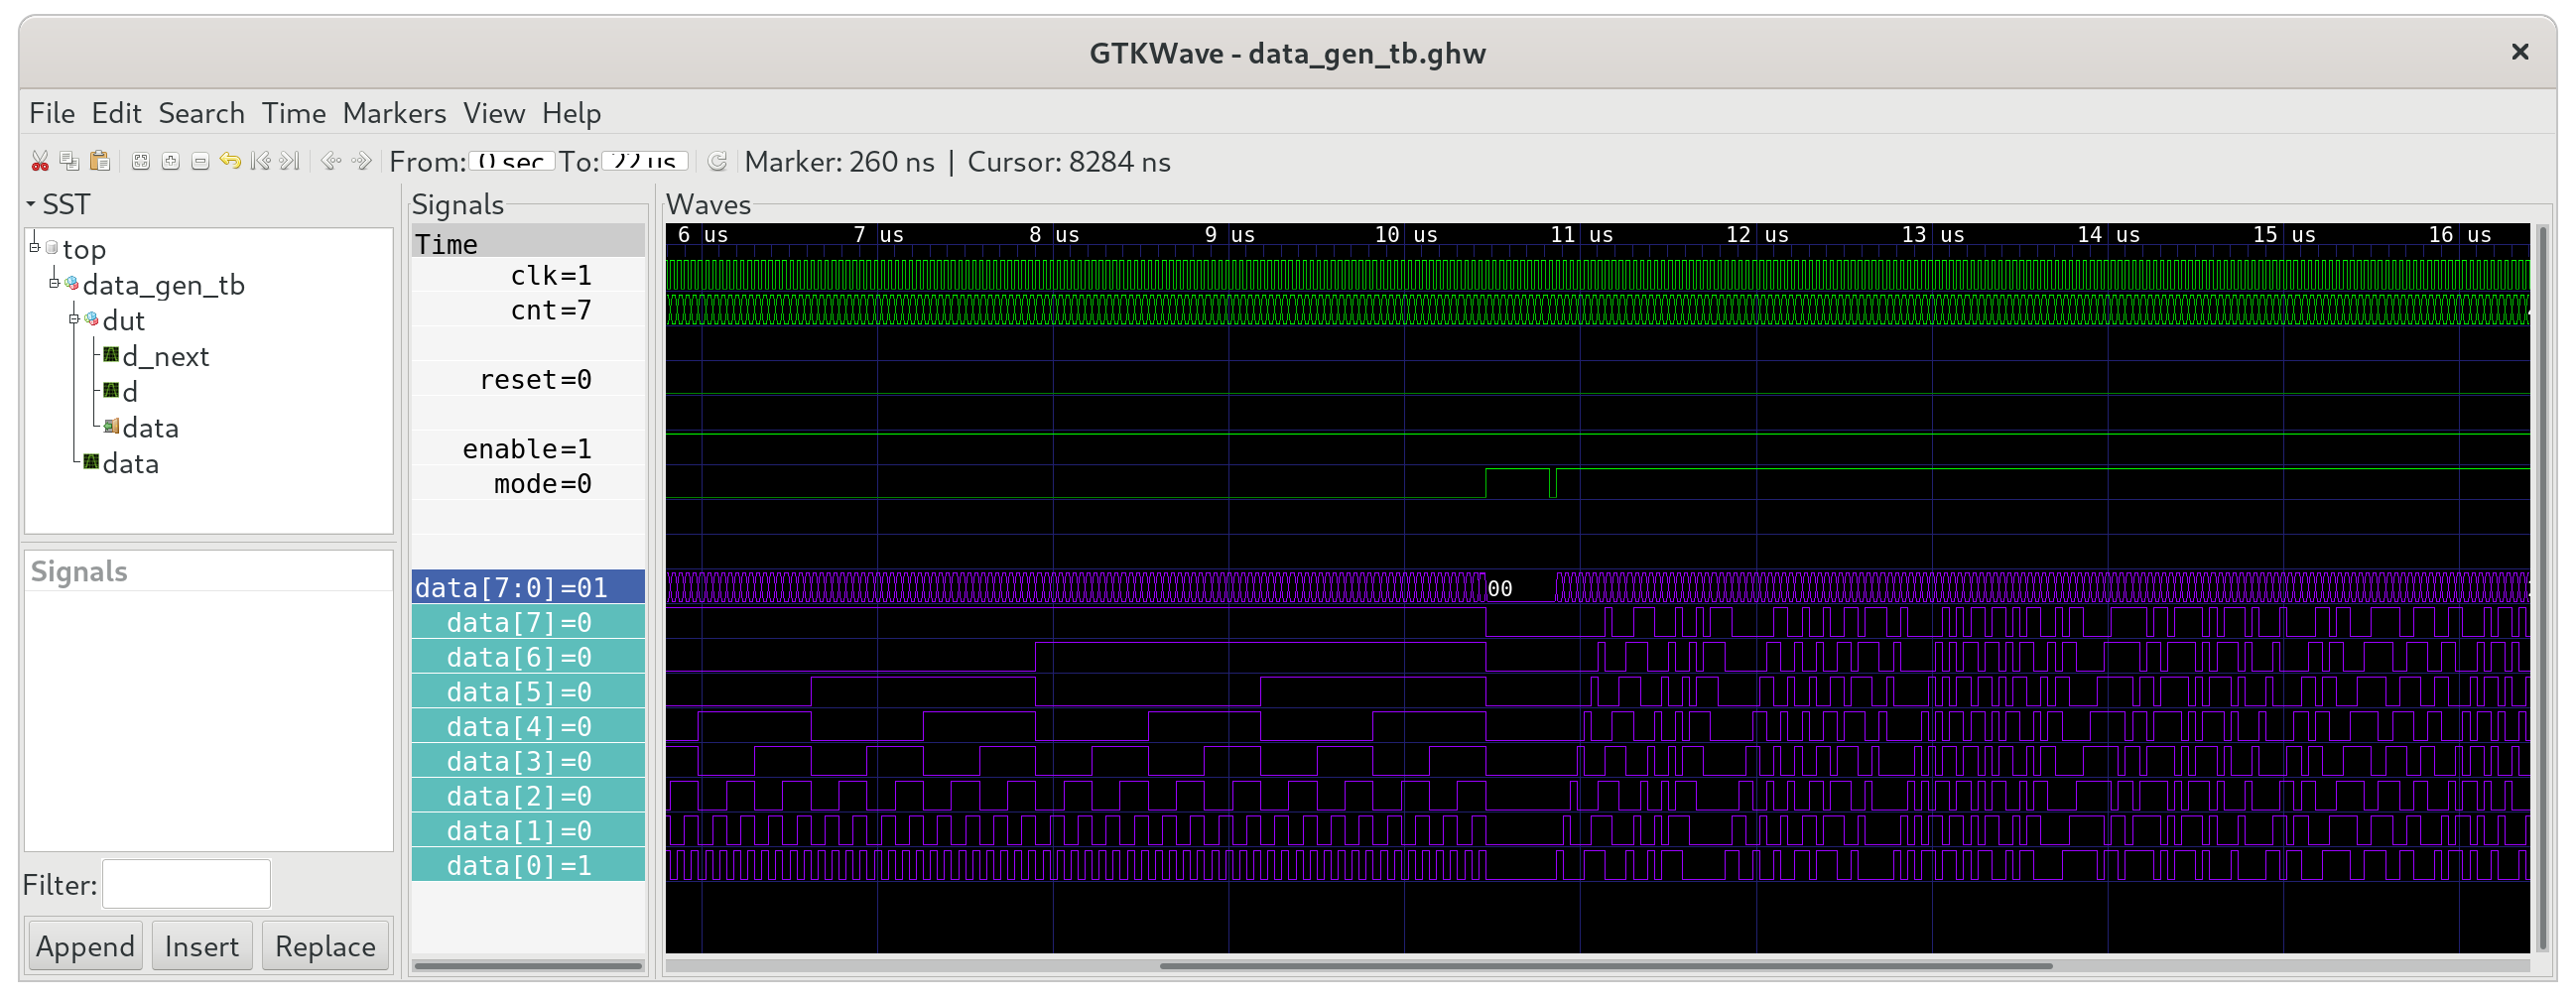
\includegraphics[width=\textwidth]{sim.png}
\end{frame}

% \section{Motivation}

\begin{frame}
  \frametitle{Logic Analyzer trace}
  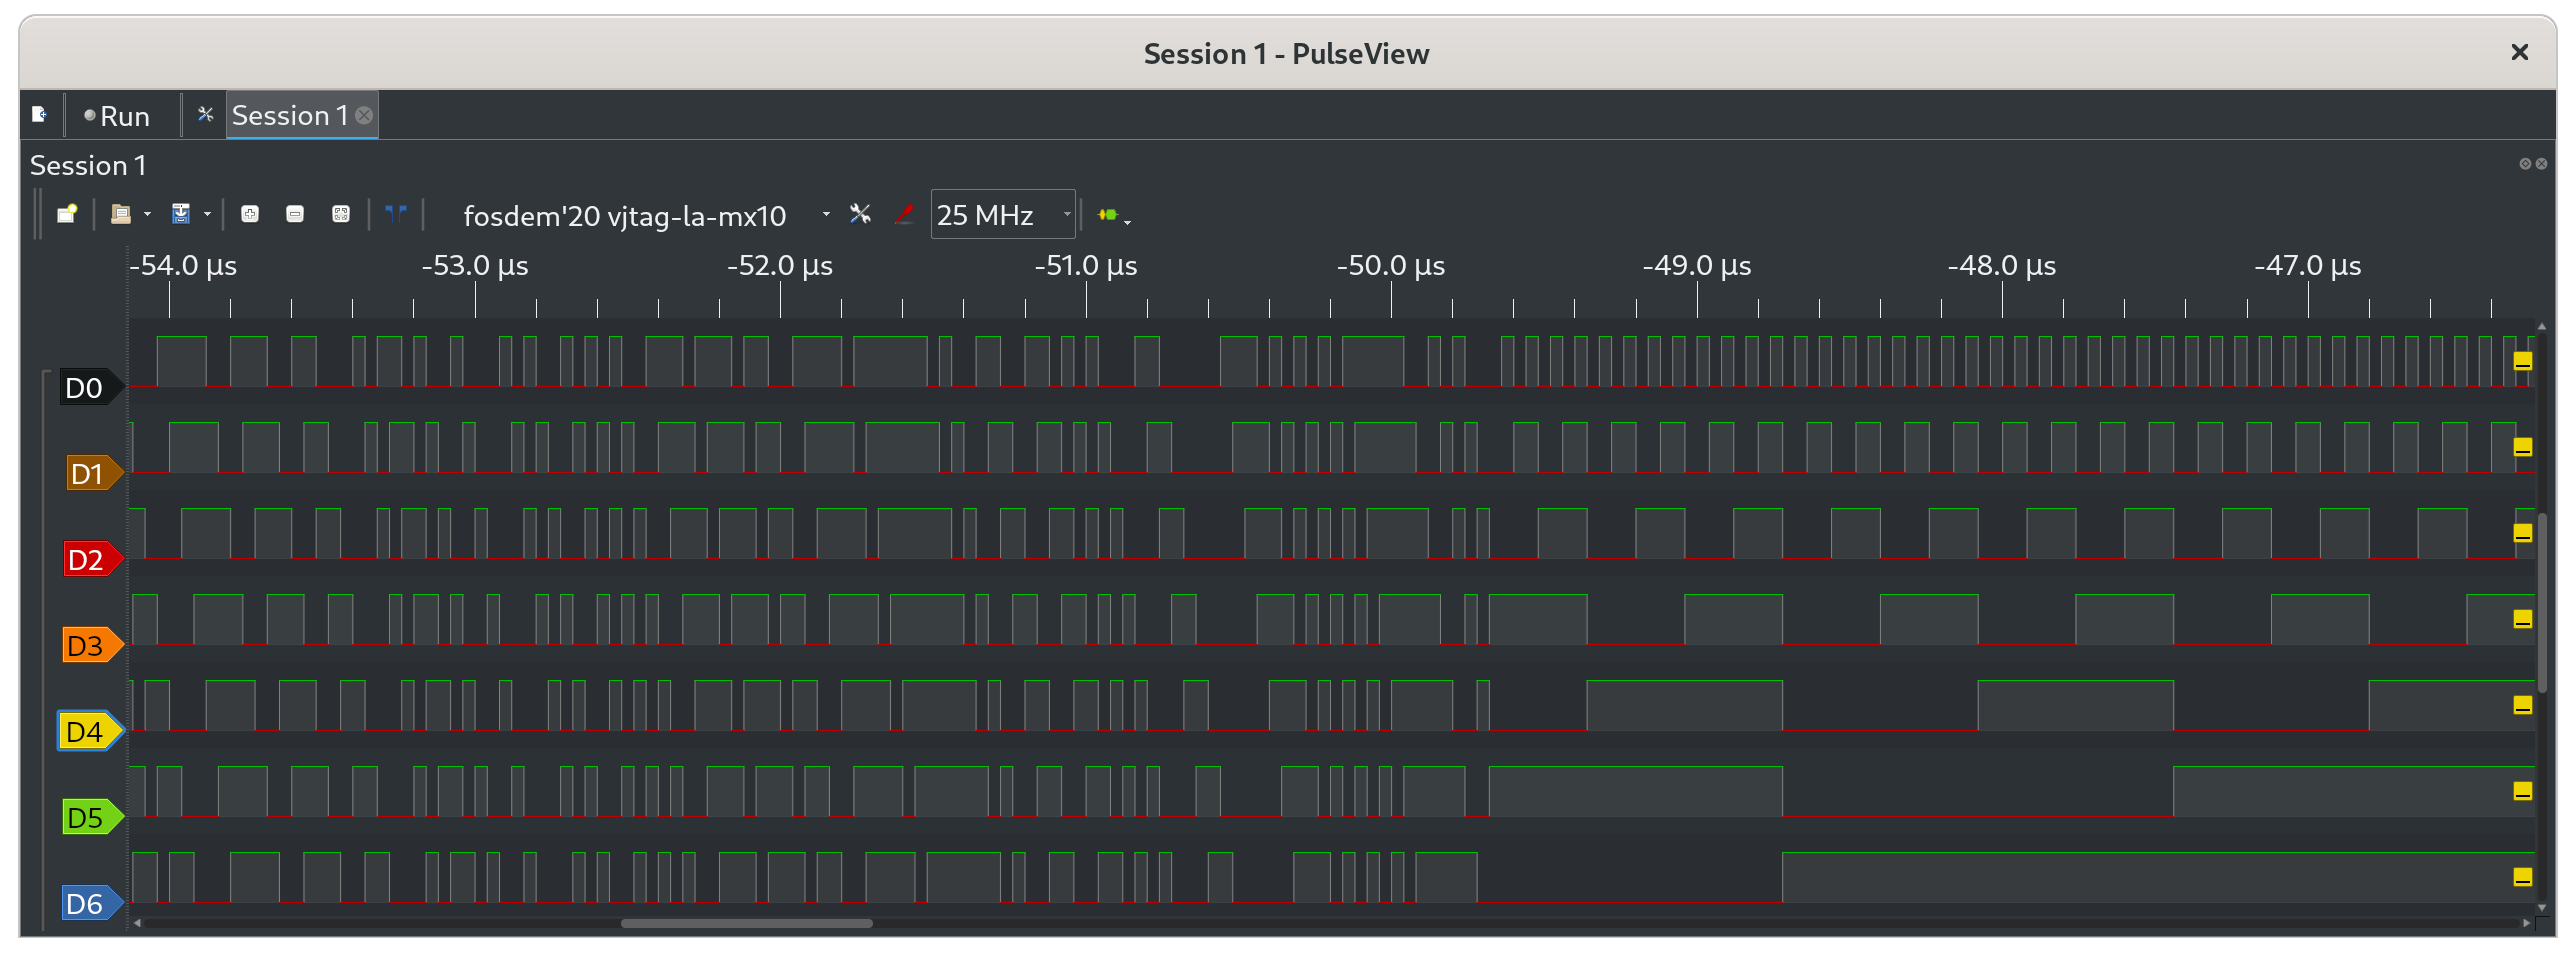
\includegraphics[width=\textwidth]{pulseview.png}
\end{frame}

% \section{luajit}

% \section{What's next\dots}

\begin{frame}
  \vskip.5cm
  \huge{Thank you!}
  \vskip2cm
  \Huge{Questions?..}
\end{frame}

\end{document}
